\documentclass[12pt]{article}
\usepackage{etex}%pour profiter pleinement du moteur pdftex.
\usepackage[utf8]{inputenc}
\usepackage[T1]{fontenc}
\usepackage[french,english]{babel}
\usepackage[babel=true]{csquotes} % csquotes va utiliser la langue définie dans babel
\usepackage{geometry}%%définir les marges
\usepackage{graphicx}
\usepackage{lmodern}% police vectorielle
\usepackage{xcolor}
\usepackage{amssymb}
\usepackage{amsmath}
\usepackage{enumitem}
\usepackage{setspace}
\usepackage{multicol}
\usepackage{fancyhdr}
\usepackage{bm}
\usepackage{lastpage}
\usepackage{afterpage}
\usepackage{tikz}
\usepackage{booktabs}
\usepackage{colortbl}
\usepackage{hyperref}
\usepackage{pdfpages}
\usepackage{listings}
\usepackage{wrapfig}
\usepackage{subcaption}
\usepackage{footnote}
\usepackage{xspace}
\usepackage{eurosym}
\usepackage{array}
\usepackage[font=small,skip=10pt]{caption}
\newcommand{\disp}{\textsc{Displayce}\xspace}
\newcommand{\Vast}{\bBigg@{5}}
\makesavenoteenv{table}
\hypersetup{hidelinks}
\geometry{
	paper=a4paper, % Paper size, change to letterpaper for US letter size
	top=3cm, % Top margin
	bottom=3cm, % Bottom margin
	left=2.5cm, % Left margin
	right=2.5cm, % Right margin
	headheight=14pt, % Header height
	footskip=1cm, % Space from the bottom margin to the baseline of the footer
	headsep=0.5cm, % Space from the top margin to the baseline of the header
	%showframe, % Uncomment to show how the type block is set on the page
}
%\parindent=0cm

%-------------LOGO Mécen
\newcommand{\MEE}{\hspace{-.25cm}{\fontfamily{pnc} \selectfont{
			\mbox{
				{\color[RGB]{52,74,88}M}
				\kern-.446em\lower.75ex\hbox{\color[RGB]{7,93,142}\'E}%
				\kern-.1427em\lower.795ex\hbox{\color[RGB]{7,93,142}c}%
				\kern-.511em\lower -.24ex\hbox{\color[cmyk]{0.85,0.43,0.37,0.08}$\mathbb{E}$}
				\kern-.38em\lower -.24ex\hbox{\color[cmyk]{0.85,0.43,0.37,0.08}n}}}}
}

\newtheorem{theorem}{Theorem}
\newcommand{\head}[2]{\multicolumn{1}{>{\centering\arraybackslash}p{#1}}{\textbf{#2}}}
\fancypagestyle{test}{
	\cfoot{
\includegraphics[width=62mm,height=12mm]{univtours-logo-droit.pdf}}}

\AddThinSpaceBeforeFootnotes
\FrenchFootnotes
\pagestyle{fancy}
\lhead{\scalefont{2}\selectfont \MEE}
\rhead{
\includegraphics[scale=0.1]{displayce.png}}
\cfoot{
\includegraphics[width=62mm,height=12mm]{univtours-logo-droit.pdf}}
\rfoot{\thepage/\pageref{LastPage}}


\newcommand{\HRule}{\rule{\linewidth}{0.3mm}}


% Default fixed font does not support bold face
\DeclareFixedFont{\ttb}{T1}{txtt}{bx}{n}{10} % for bold
\DeclareFixedFont{\ttm}{T1}{txtt}{m}{n}{10}  % for normal

% Custom colors
\definecolor{deepblue}{rgb}{0,0,0.5}
\definecolor{deepred}{rgb}{0.6,0,0}
\definecolor{deepgreen}{rgb}{0,0.5,0}

% Python style for highlighting
\lstdefinestyle{python}{
	language=Python,
	basicstyle=\ttm,
	otherkeywords={self},             % Add keywords here
	keywordstyle=\ttb\color{deepblue},
	emphstyle=\ttb\color{deepred},    % Custom highlighting style
	stringstyle=\color{deepgreen},
	frame=tb,                         % Any extra options here
	showstringspaces=false            % 
}
\lstset{language=Python}
%%%%%%%%%%%%%%%%%%%%%%%%%%%%%%%%%%%%%%%%%%%%%%%%%%%%%%%%%
%%%%%%%%%%%%%%%%%%%%%%%%%%%%%%%%%%%%%%%%%%%%%%%%%%%%%%%%%
\begin{document}
	\selectlanguage{french}
	\renewcommand*{\tableautorefname}{Table}
	%%%%%%%%%%%%%%%%%%%%%%%%%%%%%%%%%%%%%%%%%%%%%%%%%%%%%%%%%
	%%%%%%%%%%%%%%%%%%%%%%%%%%%%%%%%%%%%%%%%%%%%%%%%%%%%%%%%%
	\newgeometry{textheight=26cm,textwidth=18cm}
	\pagenumbering{gobble}%pas de numéro de page
	\thispagestyle{plain}
\begin{center}
	\textsc{\Large Master \'Economiste d'entreprise}\\[1cm]
	\hspace{-2cm}{\scalefont{7}\selectfont \MEE} \\\vspace{1.5cm}
	
\includegraphics[scale=0.29]{displayce.png} \\\vspace{1.5cm}
	%\textsc{\Large Displayce}\\\vspace{2cm}
	\HRule \\\vspace{.5cm}
	{\Huge\bfseries Pacing algorithm in DOOH}\\
	\vspace{.5cm}\HRule \\\vspace{3cm}
	
	% Author and supervisor
	
	\large{\begin{minipage}{0.4\textwidth}
			\begin{flushleft}
				\textsc{Thomas Maurice}\\\vspace{.5cm}
			\end{flushleft}
		\end{minipage}
		\begin{minipage}{0.4\textwidth}
			\begin{flushright}% \large
				\emph{Displayce} \\
				M. \textsc{Soueidan}\\\vspace{1cm}
				\emph{Université de Tours} \\
				M. \textsc{Favard}\\
			\end{flushright}
	\end{minipage}}
	% Bottom of the page
	
	\vspace{2cm}\today \\
	\vspace{2cm}
	
\includegraphics[scale=0.2]{univtours-logo-droit.pdf}\\
\end{center}
\restoregeometry
\newgeometry{headsep = 55pt, footskip = 1cm, bottom = 2cm}
\pagenumbering{arabic}%commencer numérotation
\normalsize
\selectlanguage{english}
\renewcommand{\contentsname}{Table of contents}
\tableofcontents
\newpage

\section{Introduction}

\subsection{What is Displayce?}

\disp is the first \textsc{dsp}\footnote{Demand Side Platform: a technological solution that allows you to automate the purchase of advertising inventory.} and the leading technological platform designed to optimise ad campaigns run on digital posters and billboards. It is what we called the \textsc{dooh} which stands for \emph{Digital Out Of Home}. An ad campaign's impact and quality can be optimized thanks to the programmatic purchase which falling within the scope of the open real time bidding, allows to spend an ad budget efficiently over time and space. Hence, \disp is an intermediary between supply and demand where the supply is a digital posters publisher and the demand is an advertiser. \\

Founded in 2014 by Laure Malergue, \disp is the leading \textsc{dsp} in France with access in more than 38 000 digital posters within different points of interet such as shopping malls, car parks, tobacco shops and avenues. Being the main intermediary, the platform then is of interest for both supply and demand. It allows publishers to reach multiple potential advertisers (supply side) and media agencies to benefit from a centralization of a major part of the offer (demand side). In general, it eliminates all the tedious negotiation and booking steps formerly effective. The interest in positioning itself as a \textsc{dsp} specialising in digital posters lies in the fact that the latter are becoming increasingly attractive. Indeed, their dynamic aspect, contrary to the old outdoor displays, is a force of attraction for consumers and the cost of setting up an advertisement display is practically nil. \\

\subsection{How does DOOH works?}

\disp's programmatic purchasing platform is divided into two main parts: the booking part and the \textsc{rtb} part. The main activity is located on the Booking part but the \textsc{rtb} part is evolving. 

\subsubsection{Booking and RTB}

What is called the booking part is actually the part that concerns the reservations of digital panels. The \textsc{dsp} dedicated to booking is connected to 30 000 screens spread exclusively in France. The purchase is made on the screen. When an advertiser wishes to set up its campaign on the platform, it provides information on the location of its campaign. He can then provide information such as the type of targeted panels (by type we mean the different screen sizes, ranging from small TVs in tobacco bars to large panels in shopping centres for example), points of interest (schools, cinemas etc) or he can directly specify the precise locations (such a shop in such a city) and these locations are accompanied by the possibility of setting a targeting radius (20 km around schools for example). In addition to this location information, the advertiser specifies the broadcast dates of its campaign and from that point, \disp will automatically reserve the billboards corresponding to the advertiser's criteria. \\

\begin{center}

\includegraphics[scale=0.7]{Graphs/booking_example.png}
\end{center}

The other possibility for an advertiser is to use the \textsc{rtb} part. The major difference is that this time the purchase is not made on screen but on impression, i.e. the number of people who see the advertisement (the number of people in front of the panel). The \textsc{dsp} is connected to 53,000 panels around the world. The advertiser can specify the locations but in a less precise way than the booking part and so when a campaign is created, \disp connects to the panels concerned and receives bid requests from these panels. 


\subsubsection{Digital poster operation}

As we discuss previously, \textsc{dooh} allows to display an ad on a digital poster. We are now going to explain how does it work technically. \\
Let's take the case of a single digital panel. This panel is configured in the following way: it performs a one-minute loop with 10 seconds of broadcast per ad, so there are 6 ads that run in a loop on this panel. Each ad is submitted by a textc{dsp} such as \disp. The peculiarity is that out of these 6 ads, 5 come from so-called "acquired" campaigns and one comes from a real-time auction. Acquired campaigns are generally reserved for the week and therefore this means that during a week on the same billboard every minute the same 10 second ad comes back. The last ad, the one that comes from a real-time auction, is therefore variable, meaning that every minute, the last 10 seconds for example, it will not be the same ad as the previous minute. \\

Let's now detail how the real-time auction works. To be able to participate in an auction, you must already be connected to the panel in question in order to have previously submitted the right advertising format to be displayed. Let's suppose that there are 4 \textsc{dsp} connected to a panel with 4 different ads. Just before the 10 seconds of the real-time auction ad broadcast, the panel issues a bid request to the 4 \textsc{dsp}. Actually, as \disp is the only one \textsc{dsp}, the auction is not really an auction. When \disp receive a bid request, a price depending on the number of impressions\footnote{An impression is a person looking at a panel: if in $T$ there are 4 people in front of the panel then the bid request will provide a number of impressions equal to 4.} is associated to the bid request and so we just have to answer 'yes' we could like to buy at this given price or 'no'.  

\subsection{What is a bid request?}

We talked earlier about bid requests and real-time bidding. Let's explain what this consists of. The \textsc{rtb} (Real time bidding) is a server-to-server buying process that allows inventory (ad space) to be bought and sold on a per-impression basis (where an impression is a person who sees the specific ad). It happens instantaneous through an auction that determines who gets to buy a specific impression. It happens programmatically in the same way as financial markets do. If a bid is won, the advertisers ad is immediately shown on the digital poster in the case of digital out of home. 

A bid request provides information such as the exact location of the digital poster concerned, the exact time (to the nearest millisecond), the number of people in front of the poster and sometimes even the details of these people, namely their age group and gender. In the end, this information makes it possible to buy an audience rather than a panel location, and this is what allows optimization. The real time bidding system therefore makes it possible to develop algorithms for intermediaries such as \disp in order to optimise the budget expenditure, reach the largest audience, smooth the budget in time and space for example etc.\\

My internship at \disp concerns the pacing part of the budget expenditure in order to ensure that the budget of a campaign is on the one hand completely exhausted and on the other hand spent uniformly over the day. 

\newpage

\section{Auction theory}
\subsection{Types of standard auctions}

Auctions are transactions with a specific set of rules detailing resource allocation according to participants' bids (amounts of money they are willing to pay). In game theory auctions are categorized as games with incomplete information because in the vast majority, one player will possess information that other players don't. \\
Standard auctions require that the winner of the auction be the participant with the highest bid. There are traditionally four types of auction that are used for the allocation of a single item: 
\begin{enumerate}
\item \emph{Ascending-bid auction} where the price is successively raised until only one
bidder remains and that bidder wins the item at the final price. 
\item \emph{Descending-bid auction} works in exactly the opposite way. The auctioneer
starts at a very high price, and then lowers the price continuously. The first bidder
who agrees with the current price wins the item at that price. 
\item \emph{First-price sealed-bid auction} where each bidder independently submits a
single bid, without seeing others’ bids, and the object is sold to the bidder who
makes the highest bid. The winner pays its bid.
\item \emph{Second-price sealed-bid auction} works exactly the same way as the first-price sealed-bid auction except that the price the winner pays is the second-highest bidder’s bid. This type of auction is also called \emph{Vickrey's auction}.
\end{enumerate} 
This four types can be shortened to two types. Descending-bid auction and First-price sealed-bid auctions are based on the same principles. Each bidder must choose a price to call out, conditional on no other bidder having yet called out; and the bidder who chooses the highest price wins the item at the price called out. In both case, the winner pays the bid he/she called out.
The Ascending-bid auction and the Second-price sealed-bid rest on the same principles as well but a little more reflection is needed. In an Ascending-bid auction, it is clearly a dominant strategy to stay in the bidding until the price reaches your maximum valuation of the good, that is, until you are just indifferent between winning and not winning. The next-to-last person will drop out when his/her maximum valuation of the good is reached, so the person with the highest bid will win at a price equal to the bid of the second-highest bidder. In a Second-price sealed-bid auction, a Nash equilibrium strategy is to bid the maximal valuation of the good you have, because if the worst comes to the worst you would pay your maximal valuation of the good minus $\varepsilon$ so in every case you will have a positive payoff so there is no incentive to deviate from this strategy. Here again, the person with the highest bid will win at a price equal to the bid of the second-highest bidder. Now that we can distinguish two types of standard auction from the bidder's point of view, we should ask which is the most profitable type? The answer is in the \emph{Revenue Equivalence Theorem} (Vickrey, 1961) which states  that for certain economic environments, the expected revenue and bidder profits for a broad class of auctions will be the same provided that bidders use equilibrium strategies.
\newpage

\subsection{Revenue Equivalence Theorem analysis}

\begin{theorem}
For any two Bayesian-Nash incentive compatible mechanisms, if the surplus function is the same in both mechanisms, the valuation  of each player is drawn from the same continuous distribution and each player bid their optimal strategy then the expected payments of all types are the same in both mechanisms, and hence the expected revenue (sum of payments) is the same in both mechanisms.
\end{theorem}
Let's clarify some important terms. The maximal valuation that a consumer has for a good is the maximal price he is willing to pay for this good. The consumer's surplus is the difference between the valuation that a consumer have of a good and the price he pays for this good. Namely, it is the gain of a consumer after a purchase. Finally the optimal strategy is the bid that a player should call in order to maximize his surplus. We call it as a Nash equilibrium when no deviation is worth it.\\

This part will bring a proof of the revenue equivalence theorem. To do so we will consider two standard auction mechanisms: second-price and first-price.\\
Let's assume an auction with two risk-neutral bidders and one seller. The seller sells a single item. Each bidder $i$ has a valuation $v_i$ of the good, $v_i$ is drawn independantly in a uniform distribution $[0,1]$. We study standard auction so the bidder with the highest bid wins. Bidder $i$ calls out a bid $b_i(v_i)$ that is increasing in $v_i$ so that the bidder with the highest valuation of the good wins. We recall that the revenue equivalence theorem states that if there are 2 bidders with values drawn from $U[0,1]$ then for any standard auction the winner bidder with valuation $v$ will pay in average $\frac{1}{3}$ and will have an expected surplus $\frac{1}{2}v^2$. More generally, if there are $N$ bidders with valuation from a continuous distribution, then any standard auction leads to the same expected highest bid and the same expected bidder surplus. 

\subsubsection{Second-price auction}
To evolve the proof of the revenue equivalence theorem let's study the case in the second-price auction. We will first clarify the payment rule for this auction, then we will show that the optimal strategy for each player is to bid their maximal valuation of the good noticed $v_i$ for player $i$. Next step will be to find the expected $v_i$ assuming that $v_i > v_j$ is $\frac{2}{3}$ in our framework. Finally we will deduce that the expected bid of player $i$ is $b_i^* = \frac{1}{2}v_i = \frac{1}{3}$ and the expected surplus is given by $S(v_i)^* = \frac{1}{2}v_i^2 = \frac{2}{9}$.\\

\noindent The payment rule of this auction is the following: 
\begin{itemize}
	\item if $b_i < b_j$, bidder $i$ pays $0$
	\item if $b_i > b_j$, bidder $i$ pays $b_j$
\end{itemize}
The Nash equilibrium for a Vickrey auction is that all players bid their maximal valuation for the good namely: $b_i = v_i$. It is a dominant strategy because if $v_i > v_j$ then player $i$ has a payoff equal to $v_i - v_j > 0$ because $i$ would win the auction and pays the second price namely $v_j$. Player $j$'s payoff is 0. There is no incentive to deviate for each player, indeed, if player $i$ deviates, he loses surplus. If player $j$ wants to change is payoff of 0, then he has to bid more than $v_i$ in which case the payoff would be $v_j - v_i < 0$ so neither player $i$ nor player $j$ have an incentive to deviate.\\

\noindent The equilibrium strategies for both players are: \\
$b_i^* = v_i$ \\
$b_j^* = v_j$\\
Now let's assume that $v_i > v_j$ so that player $i$ wins. The next step is to find to what $v_i$ and $v_j$ are equal. To do so we have to find the expected value of the highest draw in a uniform law $U[0,1]$.\\

Consider N independent draws from a uniform distribution over $[0, 1]$. On average, what is the highest draw?\\

Let $X_i$ be a single draw from the uniform distribution. Then it follows that it has a cumulative density function of  $$F(x) = \left\{\begin{array}{lr}
x, & 0\le x < 1,\\
1, & x = 1,\\
0, & \text{ Otherwise}. \end{array}\right.$$
For N draws, then, what we are looking for is $Y=\max(X_i)$. The cumulative density function of $Y$ is equal to $\mathbb{P}(Y\le y)$.\\
Since $Y$ is the max, no independant draw $X_i$ can be greater than $y$ thus we can write:
\begin{flalign*}
\mathbb{P}(Y\le y) =& \ \mathbb{P}(X_1\le y, X_2\le y,\ldots,X_N\le y)&\\
=& \ \mathbb{P}(X_1\le y)\mathbb{P}(X_2\le y)\ldots\mathbb{P}(X_N\le y)&\\
=& \ F(y)F(y)\ldots F(y) &\\
=& \ [F(y)]^N
\end{flalign*}
The above cumulative density function is continuous, so we can find the probability density function of $Y$ by taking its derivative: $NF(y)^{N-1}\times f(y)$ and since we are over $[0,1]$, $f(y)=1$.\\
Then reminding that $\mathbb{E}(X) = \displaystyle \int_a^b xf(x)\ dx$, we can calculate:
\begin{flalign*}
\mathbb{E}(Y) =& \ \displaystyle \int_0^1 y(Ny^{N-1})\ dy &\\
=& \ \displaystyle \int_0^1 Ny^{N}\ dy &\\
=& \ \biggl[ \dfrac{N}{N+1}y^{N+1} \biggr]_0^1
\end{flalign*}
So we obtain $$\boxed{\mathbb{E}(Y) = \dfrac{N}{N+1}}$$

\noindent Symmetrically we can obtain that on average the lowest draw is given by:\\
$$\boxed{\mathbb{E}(Y) = 1 - \dfrac{N}{N+1}}$$ \\

\vspace{.1cm}
\noindent Let's go back to our model. As we have 2 players, $N=2$ so the expected highest valuation of the good is $v_i = \dfrac{2}{3}$ and the expected lowest valuation is $v_j = \dfrac{1}{3}$ which is more generally $v_j = \dfrac{1}{2}v_i$.\\
We can see that the expected payment by the winner is as we have seen in the theorem:
$$\boxed{b_i^* = v_j = \dfrac{1}{2}v_i = \dfrac{1}{3}}$$
Now let's calculate the expected surplus of the winner. Notice that if a bidder has value $v_i$, he expects to win whenever the other bidder has a value less than $v_i$; which happens with probability equal to $v_i$. We can deduce the expected surplus:
$S(v_i) = v_i(v_i - \dfrac{1}{2}v_i)$.
$$\boxed{S(v_i)^* = \dfrac{1}{2}v_i^2 = \dfrac{2}{9}}$$
\vspace{1cm}
\subsubsection{First-price auction}
Now we need to find the expected bid and revenu of this type of auction in order to compare with the second-price auction results and so prove the revenue equivalence theorem. We will first clarify the payment rule for this auction, then we will show that the optimal strategy for each player is to bid half of their maximal valuation of the good noticed $v_i$ for player $i$. Finally we will deduce that the expected bid of player $i$ is $b_i^* = \frac{1}{2}v_i = \frac{1}{3}$ and the expected surplus is given by $S(v_i)^* = \frac{1}{2}v_i^2 = \frac{2}{9}$ exactly the same as the second price auction.\\

\noindent The payment rule of this auction is the following: 
\begin{itemize}
	\item if $b_i < b_j$, bidder $i$ pays $0$
	\item if $b_i > b_j$, bidder $i$ pays $b_i$
\end{itemize}
A first price auction with two risk-neutral bidders whose valuations are independantly drawn from a uniform distribution $U[0,1]$ has Nash equilibrium strategies: $(\frac{1}{2}v_i,\ \frac{1}{2}v_j)$. Let's proove that this equilibrium exists.\\

\noindent Assume that bidder $j$ bids $b_j = \dfrac{1}{2}v_j$, we need to find the best response $b_i$ of bidder $i$.\\
Player $i$ wins when $b_i > \dfrac{1}{2}v_j$, namely $v_j < 2b_i$. If this inequality is true, then player $i$ has a surplus equals to $v_i - b_i$. \\
Inversely, player $i$ loses when $v_j > 2b_i$ and so has a surplus equals to $0$.\\
We can then deduce the expected surplus of bidder $i$ given the strategy of bidder $j$.
\begin{flalign*}
\mathbb{E}(S_i) =& \ \displaystyle \int_0^{2b_i} (v_i-b_i)\ dv_j + \displaystyle \int_{2b_i}^1 0\ dv_j &\\
 =& \ \bigl[(v_i-b_i)v_j \bigr]_0^{2b_i} &\\
 =& \ 2v_ib_i-2b_i^2
\end{flalign*}
To find the best $b_i$ we have to maximize the expected surplus by taking its derivative and by equalizing it to $0$.\\

$\dfrac{\partial\mathbb{E}(S_i)}{\partial b_i} = 0 \Leftrightarrow 2v_i-4b_i = 0$, so we have: $b_i = \dfrac{1}{2}v_i $.\\
The best strategy of player $i$ is to bid half of his valuation, and as the game is symmetric player $j$'s best response is $\dfrac{1}{2}v_j$. \\
As shown in the second-auction case, assuming that valuations are drawn independantly from a uniform distribution and that $v_i > v_j$, the expected valuation of bidder $i$ is $v_i = \dfrac{2}{3}$. As $v_i > v_j$, bidder $i$ wins and pay its bid, so we have:
$$\boxed{b_i^* = \dfrac{1}{2}v_i = \dfrac{1}{3}}$$
The optimal bid of the winner is exactly the same under second-price and first-price auction. Here again, notice that if a bidder has value $v_i$, he expects to win whenever the other bidder has a value less than $v_i$; which happens with probability equal to $v_i$. The expected surplus will be the same as the second-price auction one:
$S(v_i) = v_i(v_i - \dfrac{1}{2}v_i)$.
$$\boxed{ S(v_i)^* = \dfrac{1}{2}v_i^2 = \dfrac{2}{9}}$$

More generally, for any given standard auction, denoting $S(v)$ the expected utility of player with a valuation $v$ of the good and $b$ the bid he called out, his surplus is the following:\\
$S(v) = v\mathbb{P}(v) - b$, so\\
$S(v)' = \mathbb{P}(v) = v$ in our context. $S(v)'$ is the probability to win the auction. Now for any standard auction, we denote $S(0)=0$, namely a bidder with the lowest possible valuation of the good make $0$ expected surplus.\\
Given a uniform distribution $U[0,1]$, the \emph{Fundamental Theorem of Calculus} gives us that:\\
$S(v) = S(0) + \displaystyle \int_0^v S(v)'\ dv = \displaystyle \int_0^v v\ dv$ which gives us the expected surplus of a bidder with valuation $v$ for any standard action.
$$\boxed{S(v) = \dfrac{1}{2}v^2} $$

\newpage
\subsection{Entry cost in Vickrey's auction}
The objective of this part is to ease the assumption that there is no entry cost in order to find the optimal bidding strategy as part of the second-price auction. The main difference with the previous analysis is that the game is now in two steps: the first step is to decide whether to participate to the auction and the second step is to define the optimal bidding strategy. \\

Let's focus on the simple case to understand the mechanism of the first step. We will see that the objective is to find a cut-off, where we decide to enter the auction. The idea is that this cut-off will be called $\tilde{v}$ and if our valuation is higher than $\tilde{v}$ then we enter, is our valuation is lower then we do not participate. \\

To find $\tilde{v}$ let's take a simple model in the case of a Vickrey's auction (second-price auction). There are two bidders whose valuations are drawn from a continuous distribution $U[0,1]$ and there is a cost equal to $F$ if we enter the auction. \\

Firstly, the objective is to find the threshold $\tilde{v}$. As $\tilde{v}$ is the minimal valuation that allows a participation, a bidder with a valuation equals to $\tilde{v}$ wins only if he is the only one to participate. He is the only one to participate only if other players have a valuation inferior to $\tilde{v}$ which happens with the probability: $\mathbb{P}(v_1<\tilde{v})\times...\times\mathbb{P}(v_{N-1}<\tilde{v})$ which is equal to $\tilde{v}^{N-1}$. We assume that the reserve price is 0. Then the bidder with valuation $\tilde{v}$ would have a payoff equals to: $\tilde{v}\times\tilde{v}^{N-1} = \tilde{v}^N$. The last step in order to find the cut-off $\tilde{v}$ is to consider the case when the bidder which has a valuation $\tilde{v}$ is indifferent between participating or not to the auction. This player is indifferent when his payoff is equal to the cost of entry, namely: $\tilde{v}^N = F$ which gives us: $\tilde{v} = F^{\frac{1}{N}}$.\\

Now that we have determine the first stage of the game, we can deduce the optimal bidding strategy in the second stage. If a player has a valuation higher than $\tilde{v}$ then the optimal strategy doesn't change with the previous case. The Nash equilibrium strategy is to bid his own valuation of the good. The solution with entry cost in a Vickrey's auction is the following:
$$b_i = \left\{\begin{array}{lr}
v_i, & v_i>\tilde{v}=F^{\frac{1}{N}},\\
\text{No entry}, & v_i<\tilde{v}=F^{\frac{1}{N}} \end{array}\right. $$\\

The very interesting thing about the cost of entry is the idea of sunk cost fallacy. The basic previous model predicts that once you have paid the entry cost you should bid the same way as you would if there were no entry cost. We can imagine that intuitively players are incitated to deduce the entry cost to the bid they wanted to call before the auction. However, the previous model show that when a bidder has paid to enter the auction, any entry fee that he might have paid should have no bearing on his bidding strategy.

\newpage

\section{Pacing}

Now that we have introduced how the digital out of home market works and explained some basics about auction theory, we will focus on the main subject of this report: a pacing algorithm. The objective of such an algorithm is to be able to smooth the advertising expenditure over a given time interval. The pacing concerns other dimensions than time, we can also consider smoothing the advertising expenditure over space but in our case we will first focus on the temporal dimension. \\

This algorithm is built into the \textsc{rtb} part of the platform. Before detailing the simulation and the algorithm itself, let's recall the current operation of a bid request in order to be able to set up a simulation framework that is as close as possible to reality. 
Each day \disp receives bid requests during the day containing information such as the precise timestamp of reception, the number of impressions and the total price of the bid request (which therefore depends on the number of impressions). There is also information about the location (and others) but we will not use those informations. When \disp receives a bid request, it passes through a series of automatic filters which depending on the information will return a response in the form of 'Yes' or 'No'. The pacing algorithm will be the last filter on the bid requests that need to be answered. If all the filters say 'Yes' then a positive response is sent to the \textsc{ssp} that have sent the bid request and within a delay ranging from 2 seconds to 15 minutes a notification is sent back to \disp. This notification confirms the purchase or cancels it. Even if the reception of bid requests can be approximately known in advance, the number of impressions is unknown and is an exogenous factor because it depends on the number of people in front of a digital panel. Consequently we will se that the estimation of the number of impressions per hour will be the key point to set up an efficient pacing algorithm. Before all, let's explain how does the simulation work.

\subsection{Simulation}
The first step in the development of the algorithm is simulation. The objective is to simulate a situation that is as close as possible to reality but with some control over the parameters in order to develop an algorithm that works in the majority of cases. The key point is to obtain a simulation that generates bid requests with a variable delay between each bid request. In the reality, this delay depends on the number of persons in front of a digital panel, namely the number of impressions. So we simulate the time between two bid requests thanks to a random variable which follows a Poisson Law of parameter $\lambda$ ($Pois(\lambda)$) where the $\lambda$ parameter can be thought of as the expected number of events in the interval. In our case the parameter $\lambda$ is then the number of seconds between two bid requests. As the number of seconds between two bid requests is not stable during the day, you should be able to set a scalable $\lambda$ parameter to simulate slowdowns (high number of seconds between two bid requests) and accelerations. To do so I decided to set per day threshold parameters and we can link them by linear interpolation in order to have an evolutive function. As each day has its own threshold parameters, each day behaves differently but every Monday for example looks the same. The simulation has been set up with the SimPy module of Python whose code can be found in the appendix.

The simulation gives us a dataframe with the following structure:\\


\begin{tabular}{lccccc}
	\toprule
	\head{1cm}{} &  \head{2cm}{ID}  & \head{2cm}{Imp- ressions } &  \head{1.5cm}{Price} &    \head{1.5cm}{Win} &  \head{2.5cm}{Seconds before response} \\
	\midrule
	2020-07-08 06:00:00 &          1.0 &                 10.0 &                  10.0 &   True &           365.0 \\
	2020-07-08 06:00:00 &          2.0 &                  1.0 &                   1.0 &   True &           361.0 \\
	2020-07-08 06:00:01 &          3.0 &                  5.0 &                     5.0 &   True &           555.0 \\
	2020-07-08 06:00:01 &          4.0 &                  1.0 &                    1.0 &   True &           645.0 \\
	2020-07-08 06:00:03 &          5.0 &                 1.0 &                      1.0 &   True &           310.0 \\
	2020-07-08 06:00:03 &          6.0 &                  2.0 &                      2.0 &   True &           355.0 \\
	2020-07-08 06:00:07 &          7.0 &                  8.0 &                    8.0 &   True &           775.0 \\
	2020-07-08 06:00:10 &          8.0 &                 3.0 &                   3.0 &  False &           653.0 \\
	2020-07-08 06:00:11 &         10.0 &                6.0 &                     6.0 &   True &           432.0 \\
	2020-07-08 06:00:11 &          9.0 &                 5.0 &                    5.0 &   True &           458.0 \\
	2020-07-08 06:00:12 &         11.0 &                  5.0 &                    5.0 &   True &           755.0 \\
	2020-07-08 06:00:13 &         12.0 &                 1.0 &                      1.0 &   True &           699.0 \\
	2020-07-08 06:00:14 &         13.0 &                  9.0 &                     9.0 &   True &             2.0 \\
	2020-07-08 06:00:15 &         14.0 &                  6.0 &                    6.0 &   True &           582.0 \\
	2020-07-08 06:00:16 &         15.0 &                 5.0 &                       5.0 &   True &            52.0 \\
	2020-07-08 06:00:18 &         16.0 &                  3.0 &                       3.0 &   True &           171.0 \\
	2020-07-08 06:00:21 &         19.0 &                   4.0 &                      4.0 &   True &           636.0 \\
	2020-07-08 06:00:21 &         18.0 &                  3.0 &                       3.0 &   True &           815.0 \\
	2020-07-08 06:00:21 &         17.0 &                   5.0 &                    5.0 &   True &           447.0 \\
	\bottomrule
\end{tabular}
\vspace{1cm}

The last two columns allow us to take into account the delay of notification after responding to a bid request. In fact, when you receive a bid request, and you want to buy it, the purchase is not immediate. The price goes into a part called committed budget a few moments later (between 2 seconds and 15 minutes) we receive a notification of response that either confirms the purchase (in this case the budget will be an actually spent budget) or rejects it and in this case the budget will not be spent. Theoretically this information doesn't change anything but it would changes the behaviour of the algorithm technically because it needed to know the state of the real expenditure each time in order to calculate fairly the remaining budget. \\

\subsection{Algorithm evolution}
Now that we have a file containing simulated data, we can start developing a pacing algorithm that we can test on the data. The fact that this data is simulated allows us to control some parameters. This control allows us to simulate extreme situations in order to test the limits of the algorithm and then find areas for improvement and finally know when it will not be effective in advance. Moreover, we also have access to a set of real data over a week in order to test the algorithm in real conditions. 

In this section we will really detail the scientific approach of building the algorithm step by step. The structure of evolution is the following: we start from the basic algorithm already implemented and we show a situation in which it is not efficient. The objective is then to find an improvement that makes it efficient and we repeat the process until we get a suitable algorithm. 

Let us recall that for the moment we are only concentrating on a temporal dimension of the distribution of the expenditure, but that in the long term we will also have to integrate the spatial dimension because in fact we receive bid requests internationally. 

\subsubsection{Hourly capping}

The algorithm already implemented at \disp is a time capping algorithm. When a campaign is launched, it is given a total budget and release dates. The algorithm will then divide the total budget into an hourly budget which will be a capping (maximum budget that can be spent per hour). If the impressions potential is high, in other words, if you receive a lot of impressions per hour, the total budget will be spent and each hour will have the same budget spent. Basically this meets the objectives of pacing. \autoref{good_cap} shows how a daily budget is spent with an hourly capping algorithm.   

\begin{figure}[h!]
	\centering
	\scalebox{0.7}{	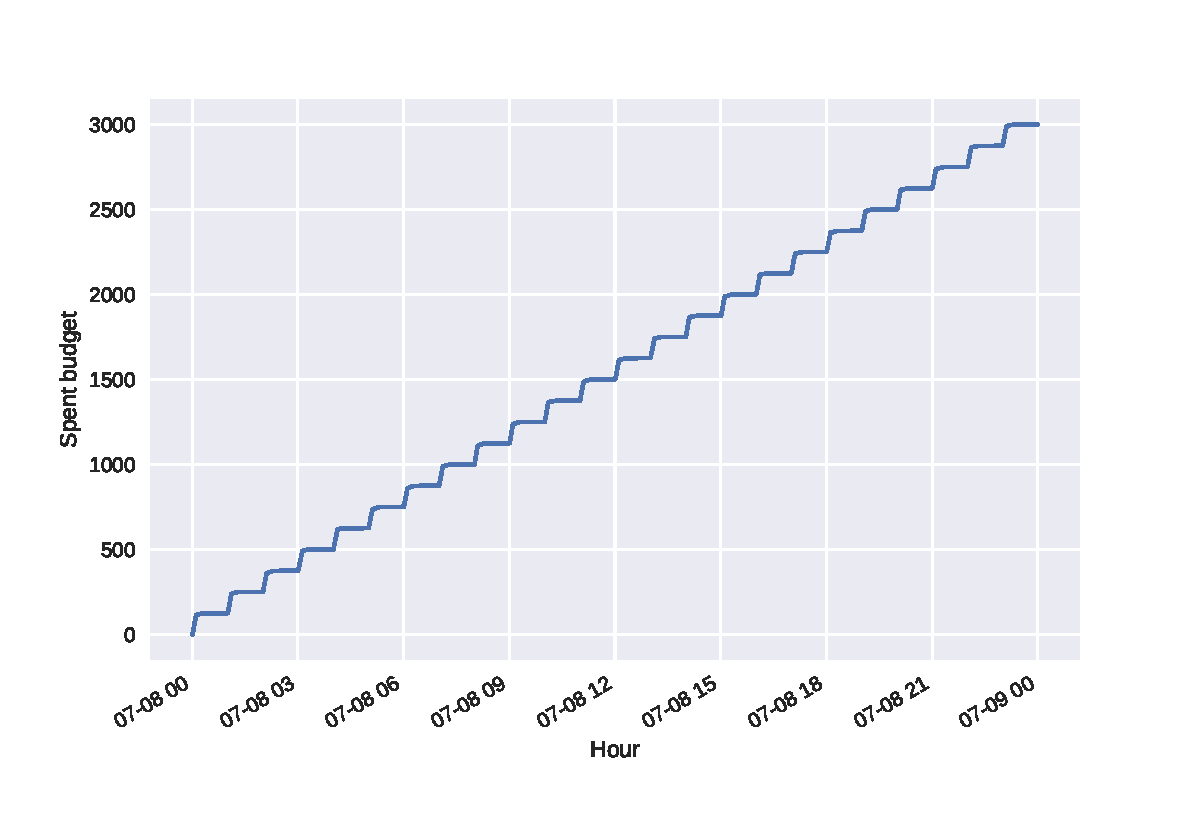
\includegraphics[scale=1]{Graphs/good_capping.pdf}}
	\caption{Spent budget over a day with capping algorithm (2020-07-08)}
	\label{good_cap}
\end{figure}

We notice that the curve is in the shape of a staircase. This phenomenon is explained by the fact that the algorithm buys as long as it has budget left to spend (the curve increases) and therefore stops buying when the hourly capping is reached (the curve remains horizontal for the rest of the hour). This is a limit of the algorithm. First of all the expenditure within each hour is not completely uniform since as long as there is budget left the algorithm systematically makes a purchase decision. If we receive a lot of impressions per hour as it is the case graphically, the algorithm will spend the entire budget for the hour on the first few minutes and will stop buying for the whole end of the hour and therefore does not guarantee uniformity. The second limitation is the situation where you don't get enough impressions to spend the whole budget in a given hour. The problem with the current algorithm is that the unspent budget of one hour will never be spent later and therefore when the campaign is finished the whole budget has not been spent and there is a surplus left. The following graph (\autoref{bad_cap}) shows that the budget spent during the day does not reach the 3000 euros of daily budget. 

\begin{figure}[h!]
	\centering
	\scalebox{0.7}{	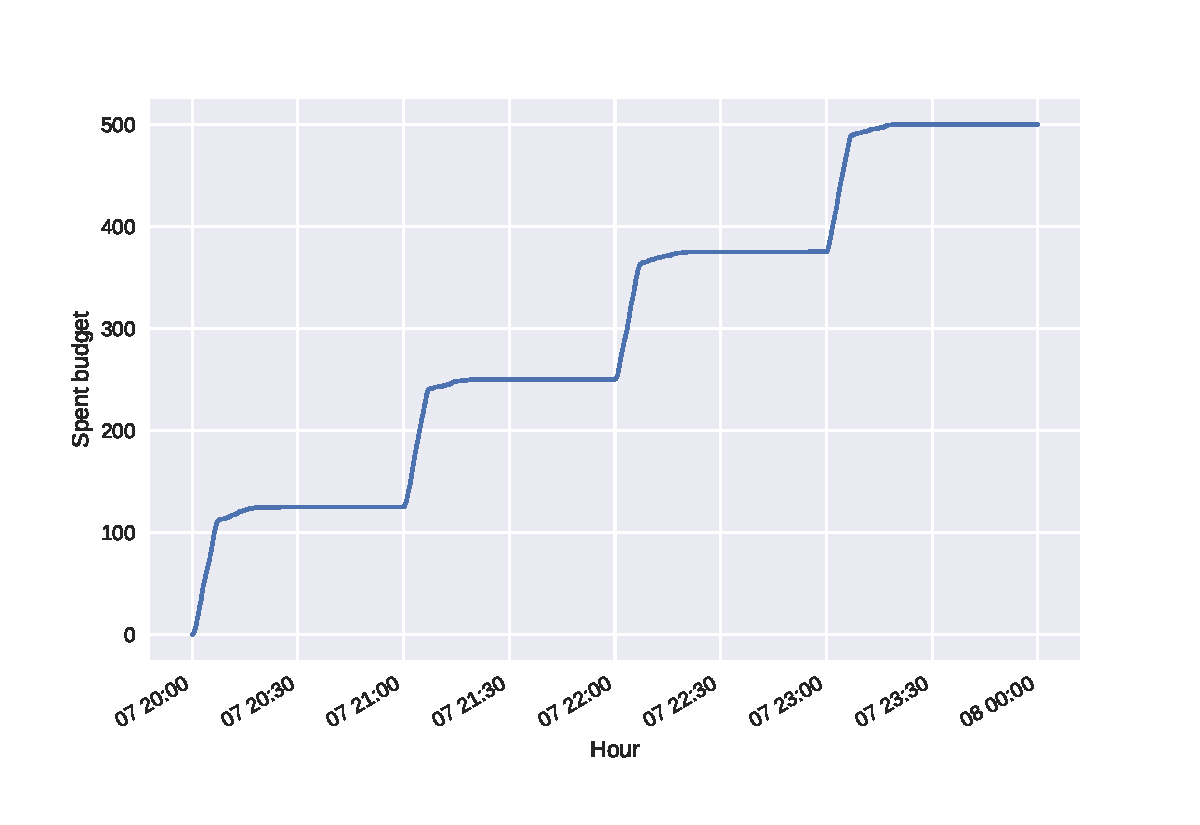
\includegraphics[scale=1]{Graphs/bad_capping.pdf}}
	\caption{Spent budget over a day with capping algorithm (2020-07-07)}
	\label{bad_cap}
\end{figure}

The curve looks exactly the same as \autoref{good_cap} but this time the curve doesn't reach the 3000 euros daily budget at the end of the day. Indeed, we can see that the spending started at 8 p.m and therefore the unspent budget from the previous hours has been definitively "lost". 

\subsubsection{Per second budget}

In order to resolve the limitations of the previous algorithm, it was decided to implement an algorithm that calculates a maximum budget per second that can be spent. Calculating this budget per second would theoretically allow a more uniform expenditure over the day and thus not end up with a stepped curve. Moreover, since the budget per second is recalculated each time a bid request is received, this allows the budget that has not been previously spent to be spent and to be freed from the constraint of the budget per hour. Given the fact that we know when the day ends, we calculate an ideal per second budget called 'target'. Then we try to keep the real expenditure per second close to this target. The idea is to have the same behaviour as a cruise control algorithm, but instead of controlling the speed we control the budget delivery. I posed the problem as a mathematically constrained optimization. The key point here is that currently we don't have a measure of quality of impressions and therefore we can't maximize on a variable that would measure the impressions' quality such as click through rate or conversion rate. Finally we can simply reduce such an optimization program to the following form:
\begin{align*}
\max_{b_t} &\quad I \\
s.c.  \qquad & 
\left\{
\begin{array}{ll} 
\displaystyle \sum_{t=1}^{T} s(t) = B\\
|s(t) - b_t | \leq \varepsilon_t\\
\end{array}
\right.
\end{align*}
Where $I$ is the number of impressions, $s(t)$ is the time expenditure $t$, $B$ is the total budget and $\varepsilon$ is a number small enough to ensure the uniformity of expenditure. The first constraint is the budget constraint, and the second constraint guarantees the objective of smoothing the expenditure in order to avoid lows or peaks of expenditure during the day. The optimization parameter is therefore $b_t$, the budget that is allocated in $t$. However, the number of impressions is exogenous, indeed the presence in front of a panel of individuals in $t$ does not depend on us. This is why at this stage the only way to guarantee a smooth expenditure over the day which thus respects the constraints presented above is to have a classic pacing algorithm which offers a budget per $t$ slice of the day. The algorithm could therefore estimate the times at which we receive bids requests and according to these times divide the day into $t$ time slots (in seconds or even more precisely) and therefore assign a budget per time slot. 
$$b_{t+1} = \Bigr(B - \displaystyle \sum_{s=1}^{t} S(s)\Bigl) \dfrac{1}{T-t}$$
where $b_{t+1}$ is the budget to be allocated to the second $t+1$, $B$ is the total budget for the day, $S(s)$ is the actual expenditure to the second $t$ and finally $T-t$ is the remaining time in seconds until the end of the day. It is important to highlight that the operation explained above is based on the estimation of the exact time of the last bid request, so that the $T-t$ calculation is precise and fair.\\ 

Since the algorithm is based on increasing the remaining budget per second when not enough impressions are received, the calculation of the budget per second can already be slightly improved by taking into account its variation. Indeed, if it increases, it means that we receive less and less impressions and therefore we buy less and consequently we should accelerate the purchase to be sure to spend the whole budget. We can therefore take into account the variation $v_t = b_t - b_{t-1}$ and the speed of the variation $a_t = v_t - v_{t-1}$. \\
The calculation of $b_t$ becomes the following:
$$b_{t+1} = \Bigr(B - \displaystyle \sum_{s=1}^{t} S(s)\Bigl) \dfrac{1 + (\bar{a}\bar{v})}{T-t}$$

Where $\bar{a}$ is the average speed in the variation of $b_t$ over the last 30 minutes and $\bar{sv}$ is the average variation of $b_t$ over the last 30 minutes as well. If $b_t$ increases more and more, $\bar{v}$ and $\bar{a}$ will increase as well, it would consequently boost the buying to catch up if we ever get less and less impressions. We can then simulate this new algorithm on the same data as the previous one and see if it better meets the objectives and thus surpasses the limits of the hourly capping algorithm. \autopageref{good_bt} shows us that the expenditure over the day is much smoother and more uniform than the hourly capping. We can notice that the expenditure curve becomes horizontal at the very end of the day. This behaviour is explained by the fact that in the calculation of the remaining time, the algorithm considers the end of the day at 11:40 pm to ensure that the entire daily budget is spent. 

\begin{figure}[h!]
	\centering
	\scalebox{0.7}{	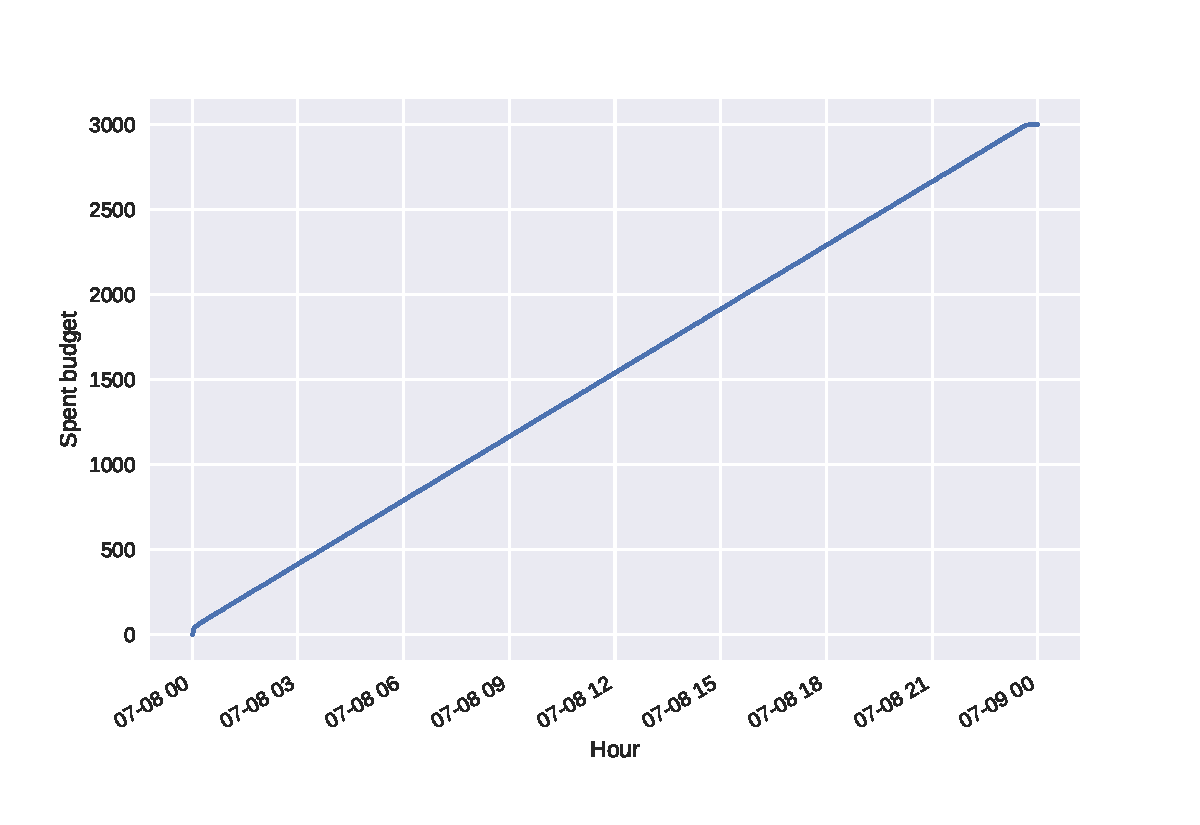
\includegraphics[scale=1]{Graphs/good_bt.pdf}}
	\caption{Spent budget over a day with budget per second algorithm (2020-07-08)}
	\label{good_bt}
\end{figure}

The second improvement of this algorithm compared to the previous one can be seen on the day the bid requests arrive at 8pm. In this configuration \autopageref{good_bt2} shows us that the unspent budget from the previous hours is caught up at the end of the day and therefore all the budget has been spent contrary to the hourly capping algorithm. We therefore conclude that the algorithm with the calculation of the budget per second is more efficient than the hourly capping algorithm. \\

\begin{figure}[h!]
	\centering
	\scalebox{0.7}{	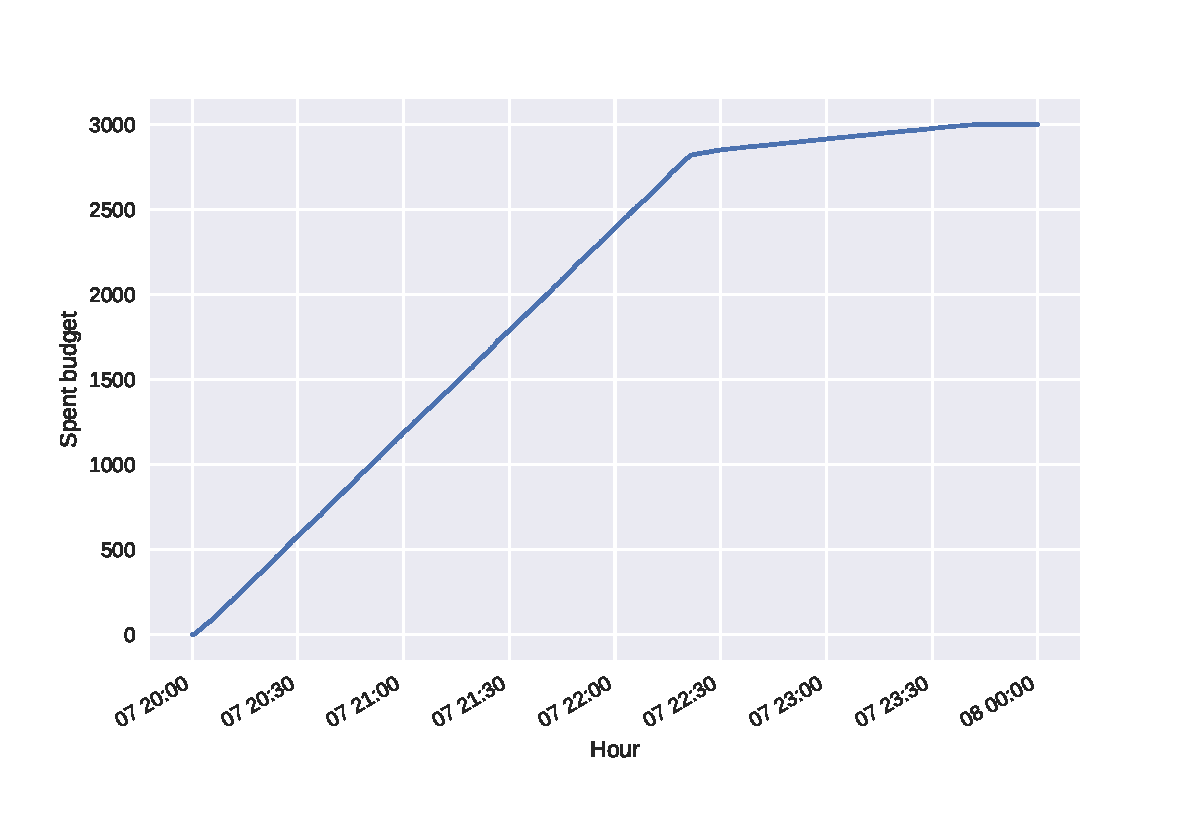
\includegraphics[scale=1]{Graphs/good_bt2.pdf}}
	\vspace{-.7cm}
	\caption{Spent budget over a day with budget per second algorithm (2020-07-07)}
	\label{good_bt2}
\end{figure}

The disadvantage of this algorithm is that when there is a backlog to catch up on, as is the case here, the algorithm will buy until it catches up and then slow down the purchase until the end of the day. It is this behaviour that explains the elbow in spending around 10:20 pm. We could then find a better way to standardize the expenditure to avoid this elbow. Despite the efficiency of this algorithm, there is another situation in which it is not efficient.

\begin{figure}[h!]
	\centering
	\scalebox{0.7}{	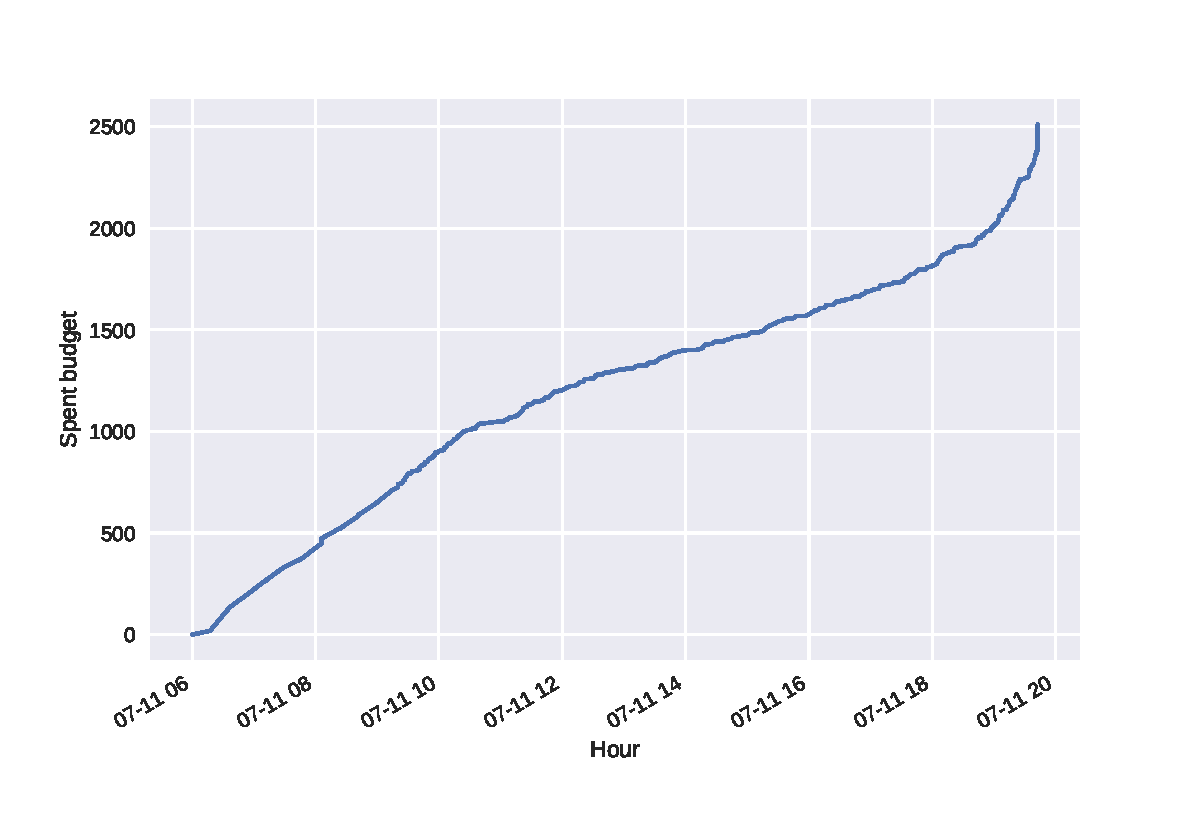
\includegraphics[scale=1]{Graphs/bad_bt.pdf}}
	\vspace{-.7cm}
	\caption{Spent budget over a day with budget per second algorithm (simulation)}
	\label{bad_bt}
\end{figure}

When there is a big slowdown in the number of impressions during the day and the number of impressions received in the remaining hours is not enough to catch up, then there will be some budget left at the end of the day. To show this situation, we can use simulated data to create a big slowdown in the course of the day. The result of the algorithm are shown in \autoref{bad_bt}. It can be seen that the slowdown could not be caught up before the end of the day and therefore the budget was not fully spent (only 2500 euros were spent).\\

\subsubsection{Evolutive hourly budget}

Although the budget per second algorithm took into account the two limitations of the time capping algorithm, we have raised two new limitations. The first one concerns the fact that the budget spent to catch up is not uniformly spent and the second one concerns the situation where there is too much slowdown in the day that cannot be caught up. The only way to deal with this is to be able to predict whether there will be a slowdown in the day. One can imagine that in the \textsc{dooh} sector, where the number of impressions depends on the number of people in front of the digital panels, each day is more or less the same and the hours when there are fewer people are perhaps predictable. The idea would then be to use historical data and perform a simple linear regression on hours of the day and days of the week to predict the proportion per hour of impressions received. If the hours with a lower proportion of impressions received are known, then a lower budget will be allocated to those hours and conversely for hours with a high proportion of impressions received. The calculation of $b_t$ then becomes:
$$b_{t+1} = \Bigr(B(h) - \displaystyle \sum_{s=1}^{t} S(s)\Bigl) \dfrac{1 + (\bar{a}\bar{v})}{T-t}$$

Where $B(h)$ is the budget allocated to the hour $h$, $\displaystyle \sum_{s=1}^{t} S(s)$ is the budget spent in the current hour $h$ and $T - t$ is the remaining number of seconds before the end of the hour $h$.

The calculation of $B(h)$ will depend on how long the campaign has been running. Indeed, on the first day we have no information on the number of impressions received during the day because we don't know which \textsc{ssp} will send bid requests nor at what time of the day they will do it. The best distribution that can be made without information in this case is a uniform distribution. From the second day a linear regression based on the data of the first day can be done to estimate the proportion per hour. This regression will therefore have the proportion of impressions as an explained variable and each hour of the day as an explanatory variable. 
$$ Prop_i = \alpha + \bm{\beta_k} \mathbf{X_k} +\varepsilon_i$$
Where $\bm{\beta_k} \mathbf{X_k}$ is the vector of coefficients associated with the vector of explanatory variables. When we have at least 7 campaign days, we can add the day of the week in the vector of explanatory variables in order to have a more accurate estimation. \\

This method therefore makes it possible to predict (if the estimation is efficient) the hours during which there is a big slowdown and thus be able to allocate a larger budget to the hours before the slowdown. In addition, the algorithm can also be improved by distributing the remaining budget of the previous hours over all the remaining hours of the day to avoid a elbow-shaped expenditure curve. 

\begin{figure}[h!]
	\centering
	\scalebox{0.7}{	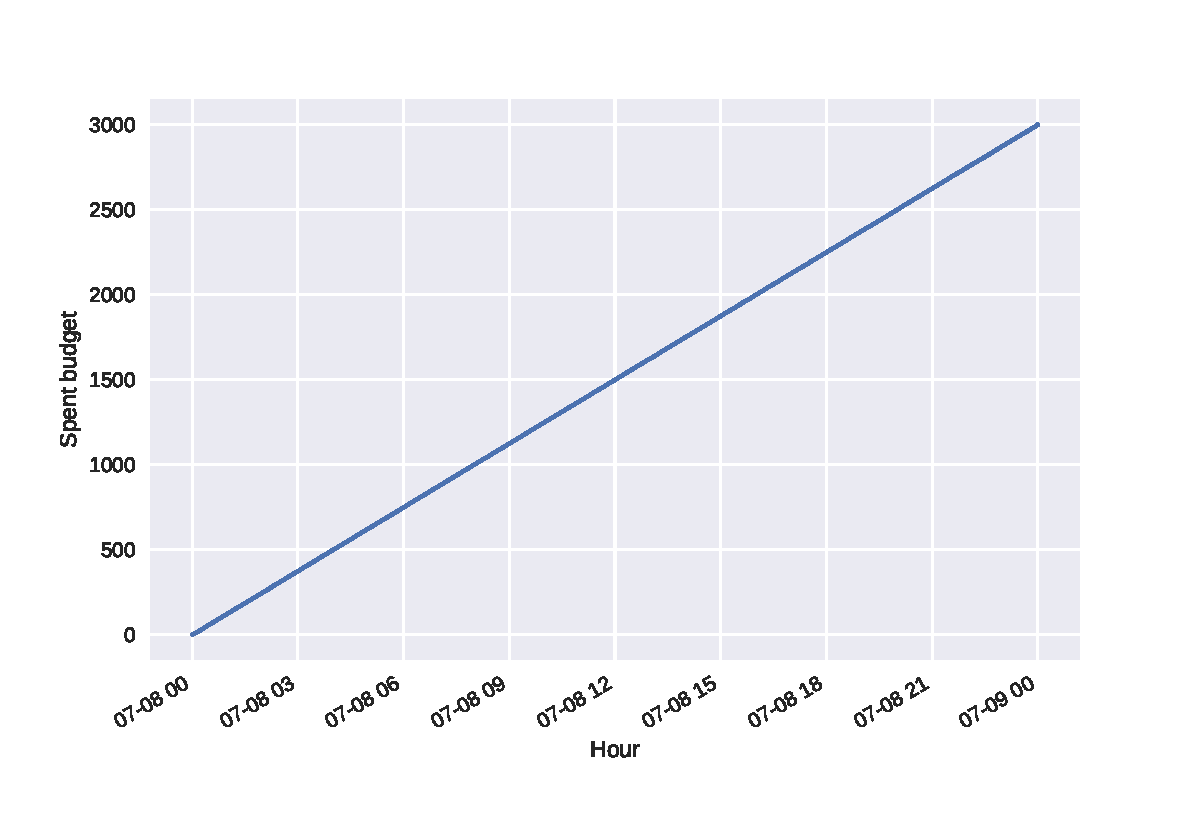
\includegraphics[scale=1]{Graphs/good_et.pdf}}
	\vspace{-.7cm}
	\caption{Spent budget over a day with hourly budget per second algorithm (2020-07-08)}
	\label{good_et}
\end{figure}

\begin{figure}[h!]
	\centering
	\scalebox{0.7}{	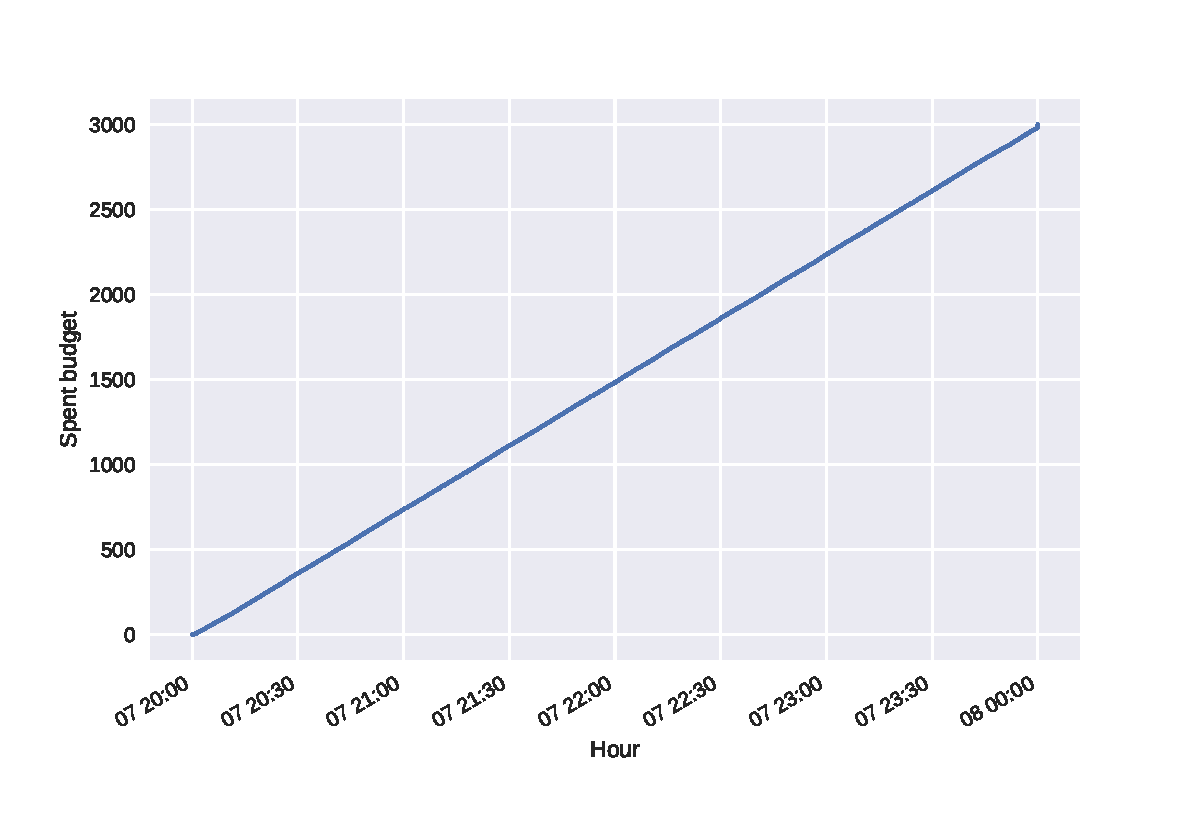
\includegraphics[scale=1]{Graphs/good_et2.pdf}}
	\vspace{-.7cm}
	\caption{Spent budget over a day with hourly budget per second algorithm (2020-07-07)}
	\label{good_et2}
\end{figure}

\autoref{good_et} gives us the same result as the previous algorithm to prove that we haven't regressed to a 'normal' situation. \autoref{good_et2} shows us that when there is a catch-up to be made, the algorithm catches up with the unspent budget much more uniformly than the previous one. There is no longer the elbow shape and all the daily budget has been spent. \autoref{spent_comparison} compare the three algorithms on the same day to see how the last one is much more efficient. The algorithm with a hourly budget per second not only makes it possible to catch up on unspent budget before the end of the day, but also the expenditure over the last hour is uniform unlike the other two algorithms. Thus, it better meets the objectives of pacing where other algorithms have limitations.

\begin{figure}[h!]
	\centering
	\scalebox{0.7}{	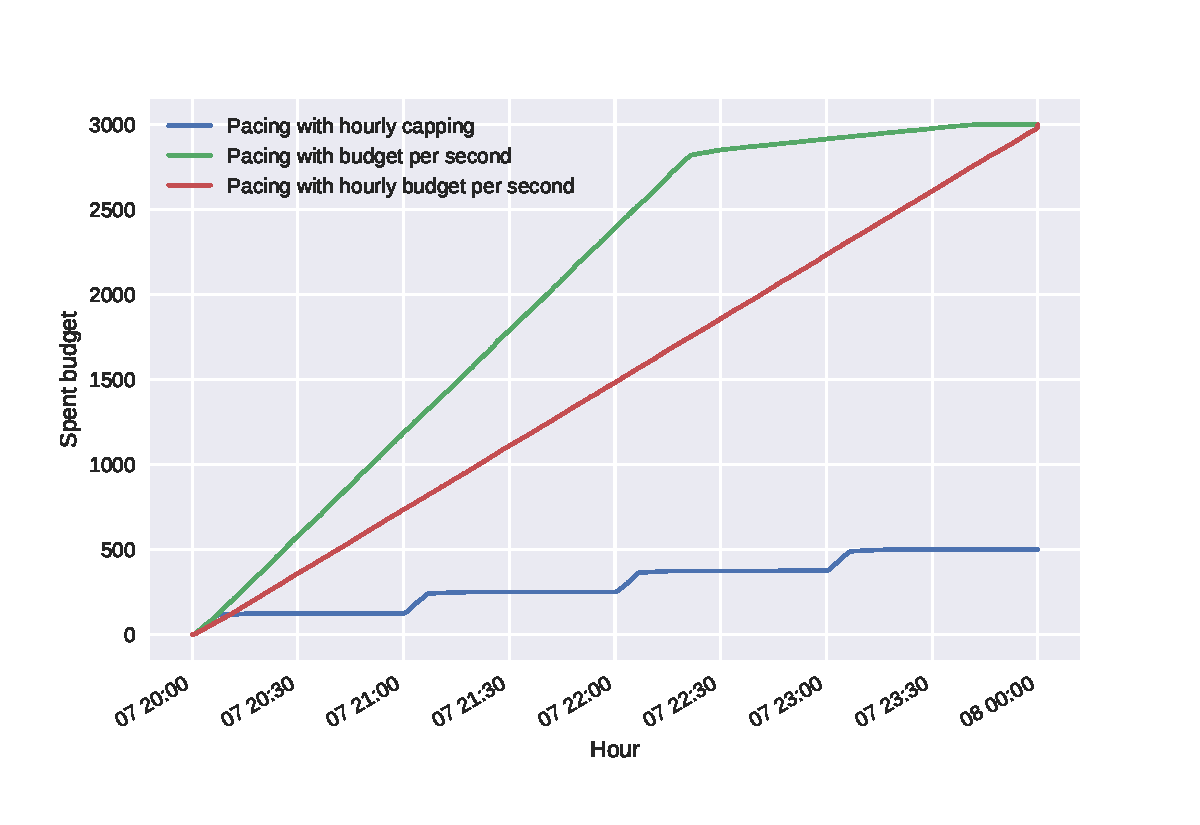
\includegraphics[scale=1]{Graphs/spent_comparison.pdf}}
	\vspace{-.7cm}
	\caption{Comparison of 3 algorithms (2020-07-07)}
	\label{spent_comparison}
\end{figure}

\newpage 

Furthermore, if we run the algorithm on simulated data, the algorithm having learned the distribution of impressions on historical data is much more efficient as shown in \autoref{good_et3}. We were able to increase spending before the slowdown and so the entire budget was spent by the end of the day.

\begin{figure}[h!]
	\centering
	\scalebox{0.7}{	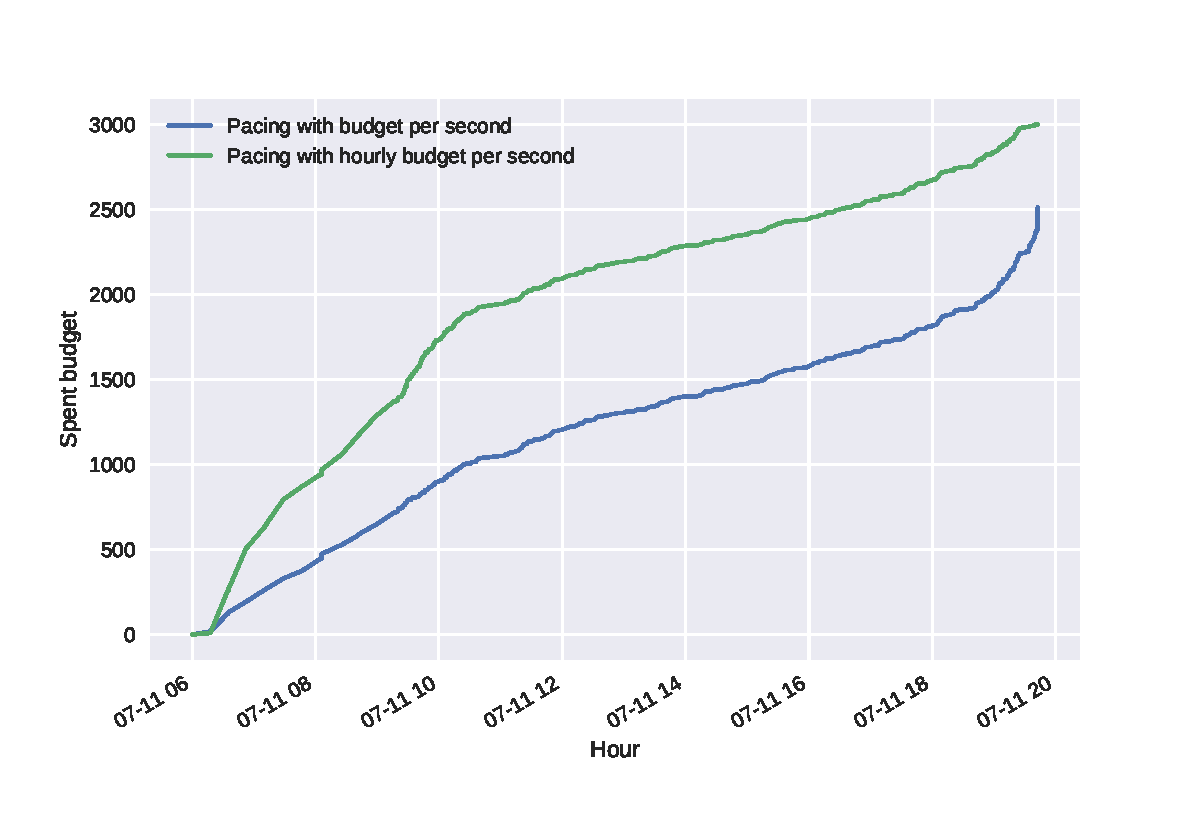
\includegraphics[scale=1]{Graphs/good_et3.pdf}}
	\vspace{-.7cm}
	\caption{Comparisons of algorithms (Simulated)}
	\label{good_et3}
\end{figure}

The budget per second per hour algorithm is more efficient than the two previous ones. However, it also has its limitations. Indeed, if a slowdown not foreseen by the estimates occurs, then it will not be efficient. Even if this aspect seems difficult or even impossible to improve, we can work on other ways to improve the algorithm. Indeed in the current state the algorithm is efficient when it receives bid requests from a single time zone. However, in reality it is necessary to integrate to the algorithm the constraint of the time-zones because with the time shift the current expenditure per hour is no longer guaranteed. We will therefore look at the spatial dimension in the next section.

\newpage


\section*{Appendix}

\begin{lstlisting}[style=Python]
#######################
## SIMULATION SCRIPT ##
#######################

import numpy as np
import random
import simpy
import csv
from collections import namedtuple
from datetime import datetime
from datetime import timedelta
from scipy.interpolate import interp1d


def imps():
	"""Function that generates the number of impressions for a br
	
	"""
	lam = int(np.random.normal(loc=4, scale=2, size=1))
	if lam < 1:
	lam = 1
	nb_imp = np.random.poisson(lam)
	return nb_imp


def delay(lam):
	"""Function that generates a number of seconds before the next br 
	following a Poisson law of lambda parameter.
	
	Arguments:
	:lam: expected number of seconds
	"""
	seconds = np.random.poisson(lam)
	# 1% probability of technical error
	if not random.random() < 0.99:
		seconds = np.random.poisson(seconds + 1000)
	return seconds


def saving(data, filename):
	"""Function to save a named tuple to CSV
	
	Arguments:
	:data: A list of named tuple to transform into CSV
	:filename: Name of the file to create
	"""
	with open(filename, "w", encoding="utf8") as file:
		# Column name for first row
		first, *_ = data
		writer = csv.DictWriter(file, first._fields)
		writer.writeheader()
		for br in data:
			writer.writerow(br._asdict())


def open_rtb(env, P, timestampnow, nb_days, bidrequests, data):
	"""Function to simulate BR with different days
	
	Arguments:
	:env: A Simpy environment
	:P: Fix price of 1 impression
	:timestampnow: Timestamp when the simulation starts
	:nb_days: Number of days to simulate
	:nb_hours_per_days: Number of opening hours of the br
	:bidrequests: A named tuple to store data
	:data: An empty list
	"""
	day = datetime.now().day
	month = datetime.now().month
	year = datetime.now().year
	next_date = datetime(year, month, day, 6, 0, 0, 0)
	setup = True
	ID = 0
	while True:
	# Are we in opening hours?
	current_hour = datetime.fromtimestamp(env.now).hour
	if 6 <= current_hour < 20:
		if setup:
		setup = False
		weekday = next_date.weekday()
		next_date += timedelta(days=1)
		# We generate different limits according to the weekday
		if weekday < 2:
			lambdas_limits = np.array([1, 5, 120, 1, 60, 2])
			timestamps_limits = np.array([env.now, env.now + 10800, 
			env.now + 21600,env.now + 28800, env.now + 43200, 
			env.now + 50400])
			f_lambdas = interp1d(timestamps_limits, lambdas_limits)
		elif 2 <= weekday < 4:
			lambdas_limits = np.array([5, 120, 1, 1, 60, 2])
			timestamps_limits = np.array([env.now, env.now + 10800,
			env.now + 21600, env.now + 28800, env.now + 43200, 
			env.now + 50400])
			f_lambdas = interp1d(timestamps_limits, lambdas_limits)
		elif 4 <= weekday < 6:
			lambdas_limits = np.array([1, 2, 180, 80, 1])
			timestamps_limits = np.array([env.now, env.now + 10800, 
			env.now + 28800, env.now + 43200, env.now + 50400])
			f_lambdas = interp1d(timestamps_limits, lambdas_limits)
		else:
			lambdas_limits = np.array([180, 1, 5, 5, 30])
			timestamps_limits = np.array([env.now, env.now + 21600, 
			env.now + 28800, env.now + 43200, env.now + 50400])
			f_lambdas = interp1d(timestamps_limits, lambdas_limits)
			
		# Generate a br
		ID += 1
		
		# Timestamp of br
		time = datetime.fromtimestamp(env.now).strftime(
		"%m-%d-%Y %H:%M:%S")
		
		# Number of impressions
		nb_imp = imps()
		price = P * nb_imp
		
		# Win/loose and number of seconds before the notification
		seconds_notif = random.randint(2, 900)
		if not random.random() < 0.95:
			win = False
		else:
			win = True
		
		# Storing data
		results = bidrequests(
			ID=ID,
			weekday=weekday,
			timestamp=env.now,
			timestamp_string=time,
			nb_imp=nb_imp,
			price=price,
			win=win,
			seconds_notif=seconds_notif
		)
		data.append(results)
		
		# Time before next BR
		time_before_next = delay(f_lambdas(env.now))
		
		# Remaining time before the end of the simulation
		rt = timestampnow + timedelta(days=nb_days).total_seconds() 
			- env.now
		
		# End of the simulation
		if rt < time_before_next:
			print(f"End of simulation at 
			{datetime.fromtimestamp(env.now)}")
		
		yield env.timeout(time_before_next)
	
	else:
		time_to_wait = datetime.timestamp(next_date) - env.now
		setup = True
		rt = timestampnow + timedelta(days=nb_days).total_seconds() 
		- env.now
		if rt <= time_to_wait:
		print(f"End of simulation at 
		{datetime.fromtimestamp(env.now)}")
		yield env.timeout(time_to_wait)


def main(year, month, day, number_of_days):
	timestampnow = datetime.timestamp(datetime(year, month, day, 6, 0, 0, 0))
	bidrequests = namedtuple(
	"bidrequests",
		(
			"ID",
			"weekday",
			"timestamp",
			"timestamp_string",
			"nb_imp",
			"price",
			"win",
			"seconds_notif"
		)
	)
	data = list()
	env = simpy.Environment(initial_time=timestampnow)
	proc = env.process(open_rtb(env=env, P=1, timestampnow=timestampnow, 
	nb_days=number_of_days, bidrequests=bidrequests, data=data))
	env.run(until=timestampnow + timedelta(days=number_of_days).total_seconds())
	saving(data, 'wd_'+str(day)+'-'+str(month)+'-'+str(year)+'.csv')


if __name__ == '__main__':
	main(2020,7,17,30)

\end{lstlisting}

\begin{lstlisting}[style=Python]
###################
## PACING SCRIPT ##
###################

from datetime import datetime
from datetime import timedelta
import pandas as pd
import uuid


class Algo:
	def __init__(self, daily_budget, prop_table):
		"""Class constructor"""
		# Fixed attributes
		self.daily_budget = daily_budget
		self.prop_table = prop_table
		# Impossible day and hour to initialize the setup
		self.day = 0
		self.current_hour = 0
		self.remaining_budget_hour = 0  # Initialize before buying
	
	def buying_decision(self, ts, price):
		"""From a BR, decide whether to buy or not
		
		Arguments:
		:ts: timestamp of the BR
		:price: price of the BR
		"""
		# TS de la BR
		weekday = datetime.fromtimestamp(ts).weekday()
		day = datetime.fromtimestamp(ts).day
		month = datetime.fromtimestamp(ts).month
		year = datetime.fromtimestamp(ts).year
		hour = datetime.fromtimestamp(ts).hour
		
		# Changement of hour
		if hour != self.current_hour:
			self.current_hour = hour
			# Evolutive target
			self.budget_hour = (self.prop_table.loc[
			hour, str(weekday)] / 100) * self.daily_budget + 
			self.remaining_budget_hour
			self.target = self.budget_hour / 3600
			self.spent_hour = 0
			
		# If we begin a new day, we reset variables
		if self.day != day:
			self.remaining_budget = self.daily_budget
			self.BT = [self.target]
			self.acceleration = pd.DataFrame({'A': 0}, 
				index=[datetime(year, month, day, 6, 0, 0, 0)])
			self.speed = [0]
			self.engaged_budget = 0
			self.spent_budget = 0
		self.day = day
		
		# Remaining time before the end of the hour
		end_hour = datetime(year, month, day, hour + 1, 0, 0, 0)
		remaining_time = datetime.timestamp(end_hour) - ts
		
		# Calculation of bt
		created_time = self.acceleration.index[-1] - timedelta(minutes=30)
		self.remaining_budget = self.daily_budget - 
		(self.engaged_budget + self.spent_budget)
		self.remaining_budget_hour = self.budget_hour - self.spent_hour
		try:
			bt = self.remaining_budget_hour * ((1 + 1 *
			 self.acceleration.A[self.acceleration.index > 
			created_time].mean()) / remaining_time)
		except ZeroDivisionError:
			bt = 1
		self.BT.append(bt)
		
		# Calculation of vt and at
		vt = self.BT[-1] - self.BT[-2]
		self.speed.append(vt)
		at = self.speed[-1] - self.speed[-2]
		self.acceleration = self.acceleration.append(
		pd.DataFrame({'A': at}, index=[datetime.fromtimestamp(ts)]))
		if (bt >= self.target) and (self.remaining_budget - price) >= 0:
			buying = True
			self.engaged_budget += price
			self.spent_hour += price
		else:
			buying = False
		
		return (buying, bt, at)
	
	def send_pending_notifications(self, current_ts=None):
		""" Send notifications
		
		:param current_ts: if None: will send all notifications, 
		else send before current_ts
		:return:
		"""
		while len(pending_notifications) > 0 and 
		(pending_notifications[0]['timestamp'] <= current_ts
		 if current_ts else True):
			ev = pending_notifications.pop(0)
			if ev['status'] == 'win':
				self.engaged_budget -= ev['br_price']
				self.spent_budget += ev['br_price']
			else:
				self.engaged_budget -= ev['br_price']
				self.spent_hour -= ev['br_price']


def main():
	data = pd.read_csv('wd_10-07-2020_08-08-2020.csv', 
	index_col="timestamp_string", parse_dates=True)
	data.index.names = ['Date']
	prop = pd.read_csv('proportion_table.csv', index_col='hour')
	pacing = Algo(daily_budget=3000, prop_table=prop)
	records = list()
	pending_notifications = list()
	day = 10
	for current_ts, row in data.iterrows():
		# Send current notifications
		pacing.send_pending_notifications(current_ts)
		if current_ts.day != day:
			day = current_ts.day
			records[-1]['engaged'] = pacing.engaged_budget
			pacing.remaining_budget = pacing.daily_budget -
			 (pacing.engaged_budget + pacing.spent_budget)
			records[-1]['remaining'] = pacing.remaining_budget
			records[-1]['spent'] = pacing.spent_budget
		
		# Receive BR
		buying, bt, at = pacing.buying_decision(row['timestamp'], 
		row['price'])
		
		# Making a decision
		if buying:
			# Buying
			next_notif_ts = current_ts + timedelta(
			seconds=row['seconds_notif'])
			status = "win" if row['win'] else "lose"
			notif_id = uuid.uuid4()
			pending_notifications.append(
			{"timestamp": next_notif_ts, "status": status, 
			'br_price': row['price'], 'id': notif_id})
			pending_notifications.sort(key=lambda x: x['timestamp'])
		record = {
		'target': pacing.target,
		'bt': bt,
		'at': at,
		'buying': buying,
		'remaining': pacing.remaining_budget,
		'spent': pacing.spent_budget,
		'engaged': pacing.engaged_budget
		}
		records.append(record)
		
	# Send remaining notifications
	pacing.send_pending_notifications()
	
	# Update last row after sending last notifications
	records[-1]['engaged'] = pacing.engaged_budget
	pacing.remaining_budget = pacing.daily_budget - 
	(pacing.engaged_budget + pacing.spent_budget)
	records[-1]['remaining'] = pacing.remaining_budget
	records[-1]['spent'] = pacing.spent_budget
	pacing_df = pd.DataFrame.from_records(records)
	new_df = pd.concat([data.reset_index(), pacing_df], axis=1,
	 ignore_index=True)
	new_df.columns = ['Date', 'id', 'weekday', 'timestamp', 
	'nb_imp', 'price', 'win', 'seconds_notif',
	'target', 'bt', 'at', 'buying', 'remaining', 'spent', 'engaged']
	new_df.set_index('Date', inplace=True)

if __name__ == '__main__':
	main()

\end{lstlisting}
\newpage
\section*{Sources}
\begin{description}
\item[https://www.cs.ubc.ca/\textasciitilde cs532l/gt2/slides/11-4.pdf:] To find the Nash equilibrium in first price auction.
\item[https://microeconomics.ca/okan\_yilankaya/spa.pdf: ] Cost entry
\item[Auctions Theory and Practice by Paul Klemperer:] To state the Revenue equivalence theorem.
\end{description}
\end{document}


